\section{Results\label{sec:assess.results}}

The results presented in this section aim at answering the research questions defined in \Cref{sec:assess.intro}.
\Cref{fig:assess.baseline} presents the performance of the global model without malicious participants to serve as a baseline to compare with.
The model displays relatively high performance on both datasets, \ie, above 0.9 for the accuracy, recall, and F1-score.
However, some classes are more challenging to detect than others.
The low representation of the ``Injection'' class in \texttt{cicids} (around 0.0017\%, see \Cref{tbl:assess.datasets}) prevents the model from learning from it, provoking this absence of evolution over time (see \Cref{fig:assess.baseline.cicids}).
The ``Infiltration'' class is more represented in the dataset (0.6108\%, approximately the same as the ``Brute Force'' and ``Bot'' classes), but remains difficult to learn because of its apparent similarity with benign traffic.
Consequently, it never exceeds a recall of 0.2.
The detection in \texttt{nb15} is better overall, with the exception of the ``Analysis'' and ``DoS'' classes that score below 0.9, although they are not the least represented classes in the dataset.

\begin{figure}[t]
  \centering
  \begin{subfigure}{.45\linewidth}
    \centering
    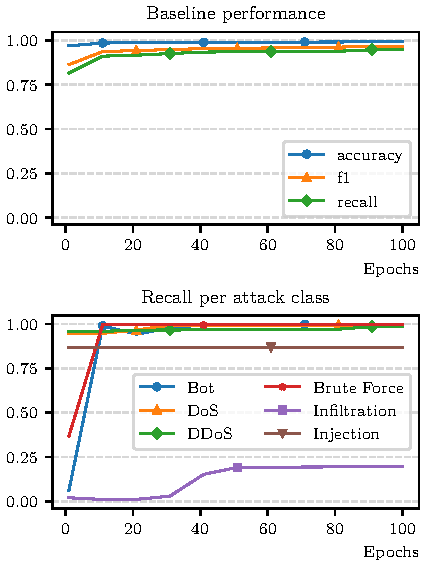
\includegraphics[width=\linewidth]{figures/cicids/baseline}
    \caption{
      CIC-CSE-IDS2018.
      \label{fig:assess.baseline.cicids}
    }
  \end{subfigure}
  \hfill
  \begin{subfigure}{.45\linewidth}
    \centering
    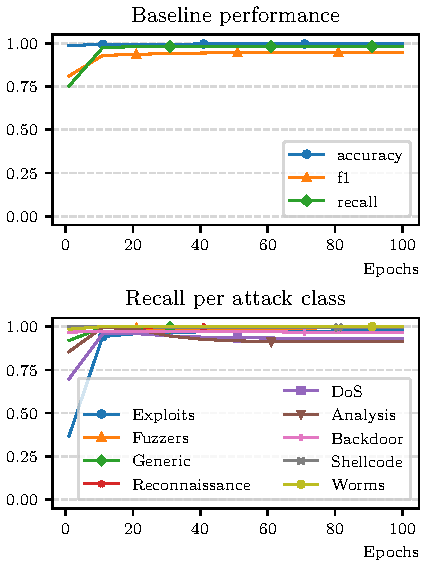
\includegraphics[width=\linewidth]{figures/nb15/baseline}
    \caption{
      UNSW-NB15.
      \label{fig:assess.baseline.nb15}
    }
  \end{subfigure}
  \caption[
    Baseline performance of the global model without malicious participants.
  ]{
    Baseline performance of the global model without malicious participants.
    The accuracy, F1-score, and recall illustrate the performance that can be expected from the global model under the conditions selected for this study ($\mathcal{E}=10$, $\beta=512$).
    The recall of the available attack classes shall serve as a reference for the \gls{rasr} of targeted attacks.
    \label{fig:assess.baseline}
  }
\end{figure}


% ------------------------------------------------------------------------------
% RQ1: PREDICTABILITY
% ------------------------------------------------------------------------------

\subsection{Impact Predictability\label{sec:assess.results.predictability}}

\begin{table}
  \caption{Experiment parameters for \ref{rq:assess.predictability}}
  \label{tbl:asssess.predictability}
  \small
  \begin{tabular}{>{\ttfamily\itshape}p{.2\columnwidth} >{\ttfamily}p{.70\columnwidth}}
    \toprule
    \multicolumn{2}{>{\bfseries}p{.9\columnwidth}}{\rqpred} \\
    \midrule
    batch\_size & 32, 512 \\
    epochs & 300\_10x30, 300\_4x75, 300\_1x300 \\
    distribution & 5-5 \\
    dataset & cicids, nb15 \\
    \bottomrule
  \end{tabular}
\end{table}

A preliminary question to answer before quantifying the effects of label-flipping is whether the behavior of poisoning attacks is predictable.
This is a requirement for generalizing our results to other datasets and models, and comparing the findings with current and future studies.
Due to computation constraints, we focus in this part on the  parameters that have the most significant impact on the results, as we need to perform longer experiments to ensure the stability of the results.
Specifically, the selected distribution contains 50\% of malicious participants (\ie, $\tau=0.5$), which roughly equates to 50\% of the training data being poisoned.
The experiments are performed during 300 epochs, with three different aggregation frequencies ($\mathcal{E} \in \lbrace 1, 4, 10 \rbrace$) and two different batch sizes ($\beta \in \lbrace 32, 512 \rbrace$).
\Cref{tbl:asssess.predictability} summarizes the parameters used for this experiment.

\begin{figure}
  \centering
  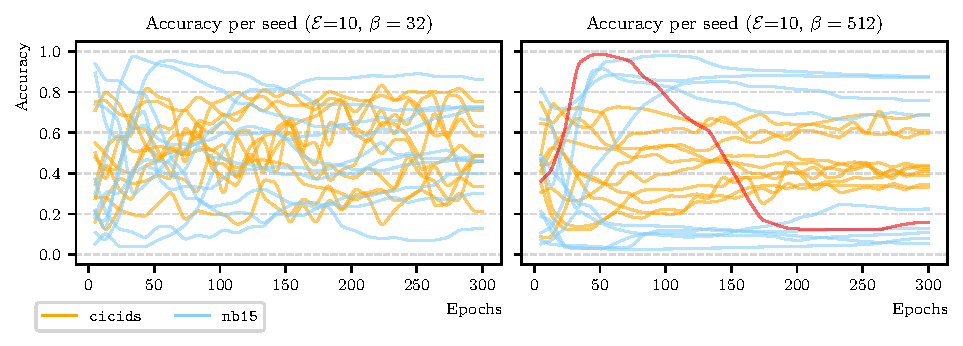
\includegraphics[width=\textwidth]{figures/accuracy_per_seed}
  \caption[
    Impact of the dataset on the accuracy under poisoning.
  ]{
    Impact of the dataset on the accuracy under poisoning.
    $\tau=0.5, \mathcal{E}=10$.
    The $x$-axis represents the number of local epochs.
    Each line represents the accuracy over time for a specific seed.
    The seed 6567 on \texttt{nb15} ($\beta=512$) is depicted in red.
    \label{fig:assess.accseed}
  }
\end{figure}

\Cref{fig:assess.accseed} illustrates the accuracy of the global model over time for each seed.
This figure brings two key insights.
First, the different runs exhibit consequent variability, especially in the early stages of training.
This is true for the runs themselves, but also for between runs on the same datasets.
Using the same parameters, the accuracy of the global model varies from 0.2 to 0.8 after 100 epochs on \texttt{cicids} (with $\beta=32$) and from 0.05 to 0.95 on \texttt{nb15}.
Some runs display particularly heterogeneous results, such as the seed 6567 on \texttt{nb15} ($\beta=512$), depicted in red in \Cref{fig:assess.predictability}, which starts below 0.4, increases to close to 1.0, before dropping below 0.2 and stabilizing.
Overall, \texttt{nb15} presents a higher variability than \texttt{cicids}, but with runs that are more stable.

\begin{figure}
  \centering
  \begin{subfigure}{\linewidth}
    \centering
    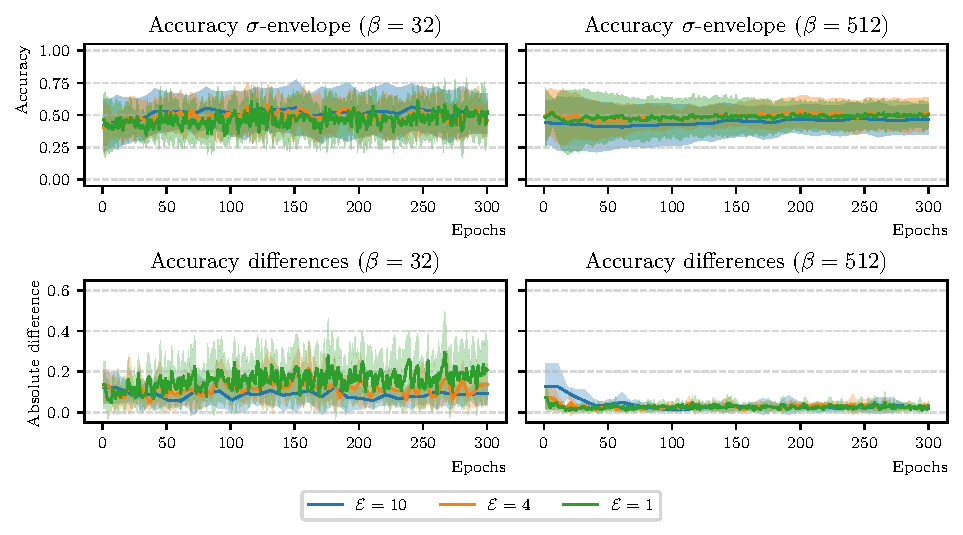
\includegraphics[width=\linewidth]{figures/cicids/predictability-all.pdf}
    \caption{
      CIC-CSE-IDS2018.
      \label{fig:predictability.cicids}
    }
  \end{subfigure}
  \begin{subfigure}{\linewidth}
    \centering
    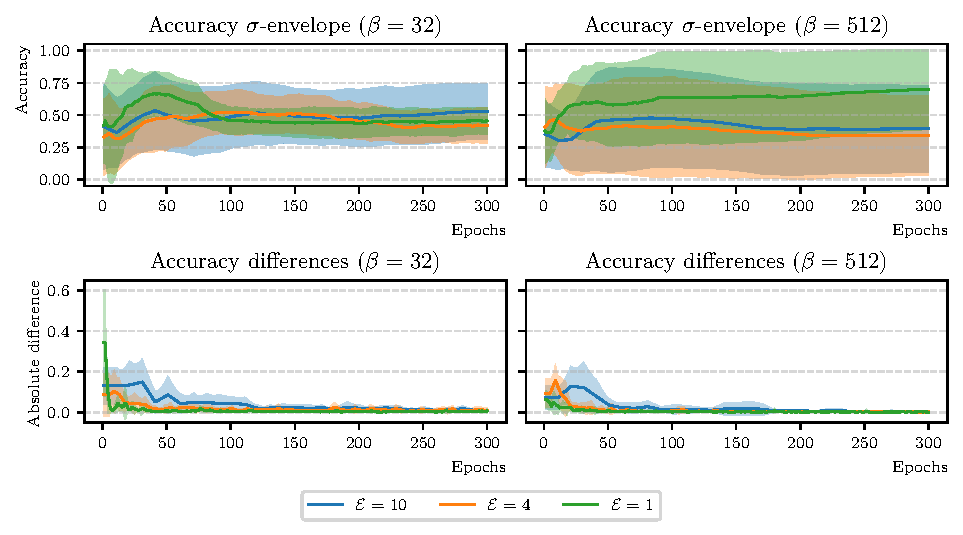
\includegraphics[width=\linewidth]{figures/nb15/predictability-all.pdf}
    \caption{
      UNSW-NB15.
      \label{fig:predictability.nb15}
    }
  \end{subfigure}
  \caption[
    Studying attack impact predictability over time.
  ]{
    Studying attack impact predictability over time, with 50\% attackers.
    The $x$-axis represents the number of local epochs.
    For each subfigure (\Cref{fig:predictability.cicids,fig:predictability.nb15}), the top row illustrates each seed's accuracy over time with its standard deviation.
    The bottom row displays the mean absolute difference ($|\text{acc}_r - \text{acc}_{r-1}|$) over time.
    \label{fig:assess.predictability}
  }
\end{figure}

The dispersion decreases over time given a big enough batch size, as shown in \Cref{fig:assess.predictability}.
More importantly, each runs progressively converges to a stedier state.
The absolute accuracy differences in the bottom rows of \Cref{fig:assess.predictability} indeed decrease over the first epochs, before plateauing.
It can be interpreted as a consequence of the complexity of the learning tasks, which becomes harder as clients possess different labels for similar samples.
Therefore, the problem probably admits a high number of local minima, which are reached depending on the seed.
On the contrary, the difference between rounds using $\mathcal{E}=32$ on \texttt{cicids} (see \Cref{fig:predictability.cicids}) tends to increase over time, illustrating the difficulty for each run to converge to a stable state.

\begin{answerbox}{Answering~\ref{rq:assess.predictability} \normalfont\itshape\rqpred}
  The behavior of poisoning attacks is not predictable, as the dispersion between results is too important, although only the seed varies.
  However, the dispersion decreases over time in some conditions, and each run tends to converge to a stable state.
  \emph{In practice, this makes the impact difficult to predict for a specific attack instance, even though general tendencies can be extrapolated.}
\end{answerbox}


% ------------------------------------------------------------------------------
% RQ2: HYPERPARAMETERS
% ------------------------------------------------------------------------------

\subsection{Hyperparameters Impact\label{sec:assess.results.hyperparams}}

\begin{table}
  \caption{Experiment parameters for \ref{rq:assess.hyperparams}}
  \label{tbl:asssess.hyperparams}
  \small
  \begin{tabular}{>{\ttfamily\itshape}p{.2\columnwidth} >{\ttfamily}p{.7\columnwidth}}
    \toprule
    \multicolumn{2}{>{\bfseries}p{.9\columnwidth}}{\rqparams} \\
    \midrule
    batch\_size & 32, 128, 512 \\
    epochs & 100\_10x10, 100\_4x25, 100\_1x100 \\
    distribution & 10-0, 5-5 \\
    scenario & continuous-100, late-3, redemption-3 \\
    \bottomrule
  \end{tabular}
\end{table}

To understand the impact of hyperparameters on the behavior of poisoning attacks, we study the impact of different batch sizes ($\beta$) and aggregation frequencies ($\mathcal{E}$).
We set again the conditions from \Cref{sec:assess.results.predictability} but limit the number of epochs to 100, as most scenarios do not show significant changes after this point (see \Cref{sec:assess.results.predictability}).
Additionally, we evaluate the hyperparameters on the \emph{late} poisoning scenario, where the attackers only start after a 3-rounds bootstrap period, and in the \emph{redemption} scenario, where the attackers stop after 3 rounds.
The experiment parameters are summarized in \Cref{tbl:asssess.hyperparams}.

\begin{figure}
  \centering
  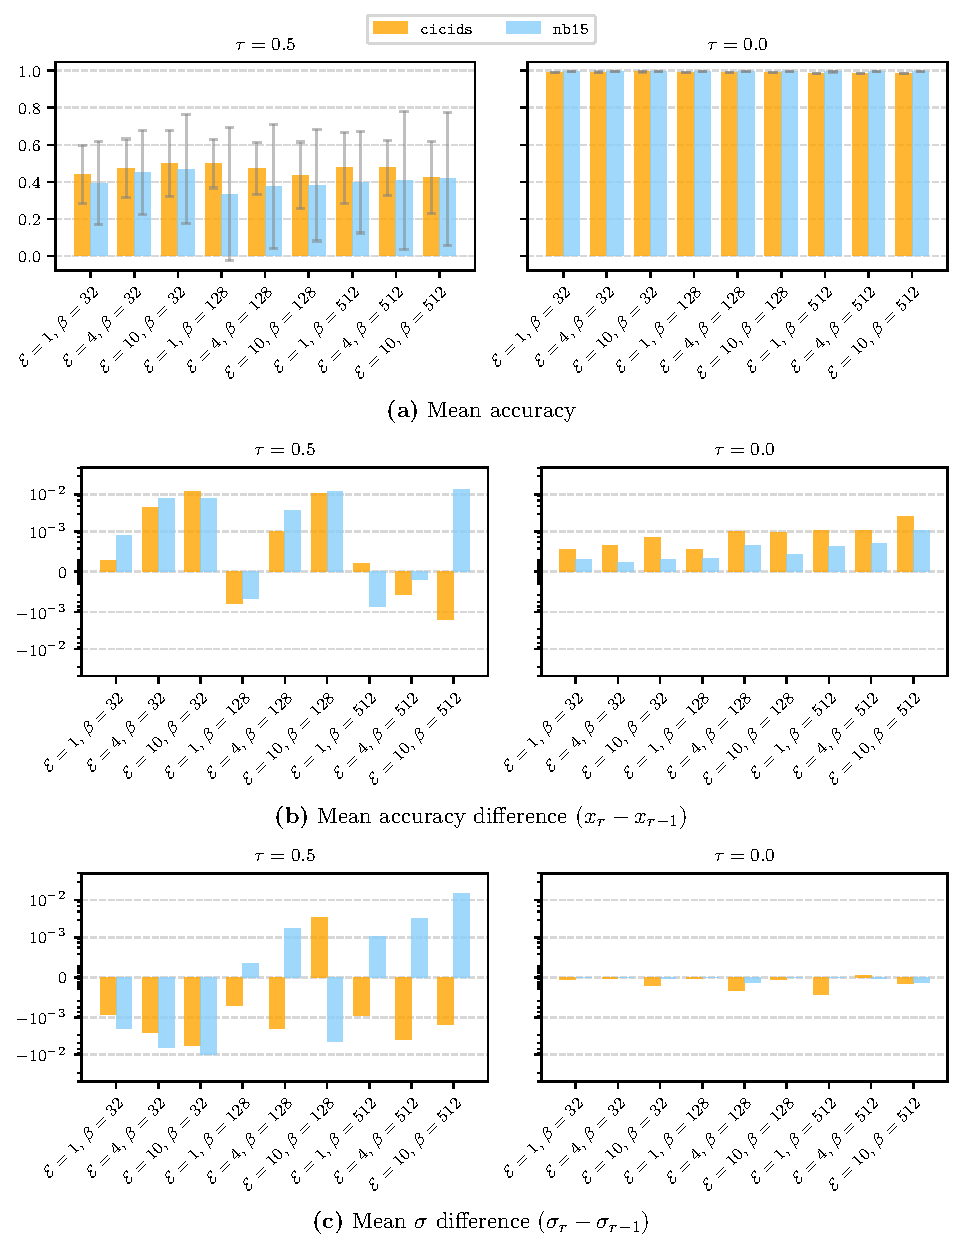
\includegraphics[width=\linewidth]{figures/hyperparams-continous.pdf}
  \caption[
    Comparing the influence of hyperparameters on the impact of label-flipping attacks.
  ]{
    Comparing the influence of hyperparameters on the impact of label-flipping attacks ($\tau \in \lbrace 0, 0.5 \rbrace$ and $\alpha=1$).
    The $x$-axis represents the number of local epochs.
    The top row illustrates the mean accuracy for each combination of hyperparameters ($\beta$ and $\mathcal{E}$).
    The middle row displays the mean difference in standard deviation ($\sigma$) between rounds.
    The bottom row shows the mean difference in terms of accuracy between rounds.
    \label{fig:assess.hyperparams-continuous}
  }
  \phantomlabels{fig:assess.hyperparams-continuous}{c}
\end{figure}

\Cref{fig:assess.hyperparams-continuous} illustrates the influence of hyperparameters on the impact of poisoning attacks.
The differences (the two bottom rows) are shown on a bi-symmetric logarithmic scale~\cite{webber_bisymmetriclogtransformation_2012}, defined as 
\begin{equation}
  x' \mapsto \text{sgn}(x) \cdot \text{log}_\text{10}(1+|\frac{x}{10^{-4}}|),
\end{equation}
to make up for the consequent differences in scale between combinations.
In addition to the accuracy of each parameter combination, \Cref{fig:assess.hyperparams-continuous} also presents the average change in standard deviation, or 
\begin{equation}
    \frac{1}{R-1}\sum_{r=2}^{R} \sigma^r - \sigma^{r-1},
\end{equation}
where $R$ is the number of rounds and $\sigma^r$ is the standard deviation of the accuracy at round $r$ between the different seeds.
The average change accuracy is also displayed.
For these metrics, a positive value indicates an increase in the observed metric over time.

In the continuous scenario studied in \Cref{fig:assess.hyperparams-continuous} (with $\tau=0.5$ and $\alpha=1$), the hyperparameters have little impact on the global model's accuracy.
Yet, $\beta=32$ presents a slight increase in accuracy over time (\Cref{fig:assess.hyperparams-continuous.b}) and a decrease in the dispersion (\Cref{fig:assess.hyperparams-continuous.c}).
Note that there is close to no dispersion in the accuracy of the benign scenario, as depicted in \Cref{fig:assess.hyperparams-continuous.c}, confirming that the attack is indeed responsible for the dispersion observed in \Cref{sec:assess.results.predictability}.
Interestingly, the correlations between the two tested datasets are more pronounced with smaller batch sizes, as shown in \Cref{fig:assess.hyperparams-continuous.b,fig:assess.hyperparams-continuous.c} where the results become less correlated with $\beta=512$.

The other hyperparameters do not display any significant correlation.
In the end, all tested parameters lead to between 0.4 and 0.5 accuracy under poisoning, while they all exceed 0.95 without poisoning.
This is critically low for intrusion detection: 0.5 is the score of a random classifier on a balanced binary-classification task.
\emph{Tossing a coin would yield better results.}

\begin{figure}[t]
  \centering
  \begin{subfigure}{.49\linewidth}
    \centering
    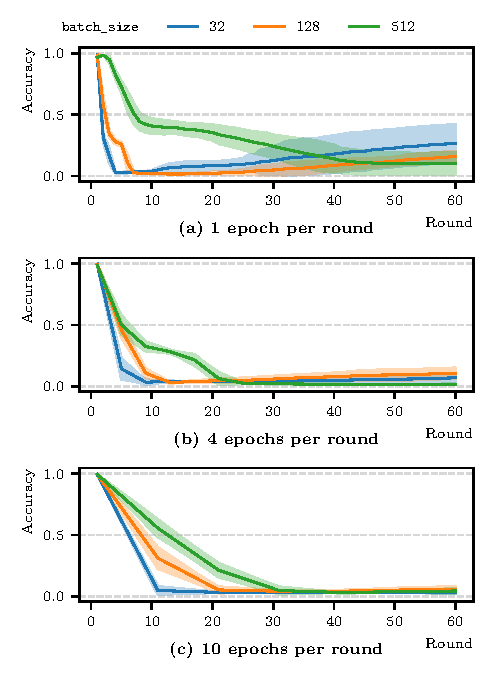
\includegraphics[width=\linewidth]{figures/cicids/hyperparams-late}
    \caption{
      CIC-CSE-IDS2018.
      \label{fig:assess.hyperparams-late.cicids}
    }
  \end{subfigure}
  \hfill
  \begin{subfigure}{.49\linewidth}
    \centering
    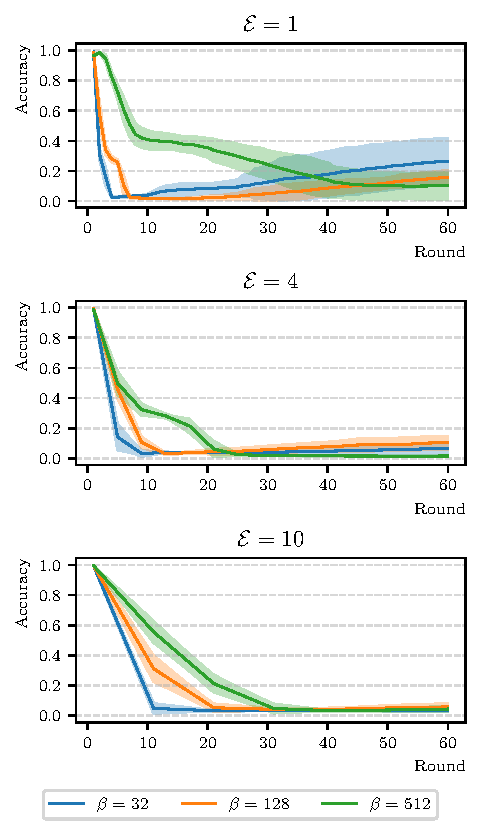
\includegraphics[width=\linewidth]{figures/nb15/hyperparams-late}
    \caption{
      UNSW-NB15.
      \label{fig:assess.hyperparams-late.nb15}
    }
  \end{subfigure}
  \caption[
    Impact of hyperparameters on the accuracy of the global model under the \texttt{late} scenario.
  ]{
    Impact of hyperparameters on the accuracy of the global model under the \texttt{late} scenario.
    The data is aligned to start at the last benign round before the attack, and the impact is measured over the next 60 epochs (\ie, 6, 24 or 60 rounds depending on the aggregation frequency).
    \label{fig:assess.hyperparams-late}
  }
\end{figure}

\begin{figure}
  \centering
  \begin{subfigure}{.49\linewidth}
    \centering
    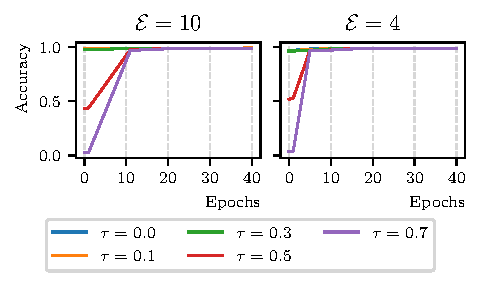
\includegraphics[width=\linewidth]{figures/cicids/redemption}
    \caption{
      CIC-CSE-IDS2018.
      \label{fig:assess.hyperparams-redemption.cicids}
    }
  \end{subfigure}
  \hfill
  \begin{subfigure}{.49\linewidth}
    \centering
    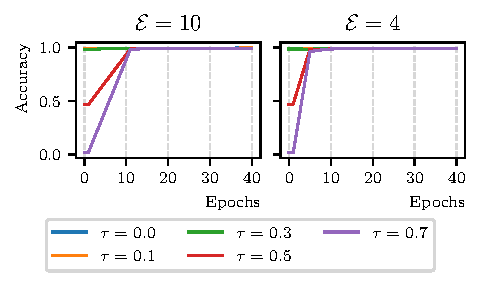
\includegraphics[width=\linewidth]{figures/nb15/redemption}
    \caption{
      UNSW-NB15.
      \label{fig:assess.hyperparams-redemption.nb15}
    }
  \end{subfigure}
  \caption[
    Accuracy of the global model after a label-flipping attack.
  ]{
    Accuracy of the global model after a label-flipping attack.
    The data is aligned to start at the last epochs before the attack ends, and the impact is measured over the next 40 epochs (\ie, 4 or 10 rounds depending on $\mathcal{E}$).
  }
  \label{fig:assess.hyperparams-redemption}
\end{figure}

However, when clients have been given the time to converge before the attack, the impact of the hyperparameters becomes more visible, particularly for the batch size as depicted in \Cref{fig:assess.hyperparams-late}.
While the impact is instantaneous when $\beta=32$, it takes around 20 epochs with $\beta=512$ to reach the same accuracy.
The dispersion of the results is significantly lower in the latter, as is the reached accuracy, which goes down to 0.25 after 60 epochs.
A bigger batch size thus leads to a greater inertia and a lower dispersion of the results when the attack starts, but also to a lower accuracy afterward.
A similar could be observed with the \texttt{redemption} scenario, where the attack stops after 3 rounds.
However, \Cref{fig:assess.hyperparams-redemption} presents a quasi-instantaneous recovery of the global model's accuracy after the attack ends.
This is expected, as \Cref{fig:assess.baseline} indicates that the global model's accuracy already exceeds 0.95 at the first round, in spite of the randomly initialized model parameters provided by the server before the first round.
This is also consistent with the results of \textcite{zhang_Evaluationdatapoisoning_2022} on NSL-KDD~\cite{tavallaee_detailedanalysisKDD_2009} and UNSW-NB15~\cite{moustafa_UNSWNB15comprehensivedata_2015}.


\begin{answerbox}{Answering~\ref{rq:assess.hyperparams} \normalfont\itshape\rqparams}
  While the hyperparameters have an impact on the poisoning effect, no combination prevents it: \emph{on average, the performance remains the same.}
  The results' dispersion can vary significantly depending on parameter combinations, especially when the attack occurs after the clients have converged.
  Then, a smaller batch size leads to a swifter effect, while a bigger batch size leads to a greater \gls{asr}.
  \emph{Therefore, in performance-constrained use cases (such as the \gls{iot}), defense mechanisms might need to react faster to mitigate the attack's impact.}
  Round-based defenses should be less affected, but history-based defenses could be significantly impacted.
  When the attack stops, the global model's accuracy recovers almost instantaneously.
\end{answerbox}


% ------------------------------------------------------------------------------
% RQ4: BACKDOORS
% ------------------------------------------------------------------------------


\subsection{IDS Backdoors using Label-flipping\label{sec:assess.results.backdoors}}

One of the main concerns with poisoning attacks is the perspective of backdoors in the \gls{ids}, allowing attackers to bypass the system's detection capabilities afterward.
To assess this risk, we study the impact of label-flipping attacks with different targets.
We consider $\alpha=100\%$ and various values of $\tau$ to assess whether a \gls{asr} of 1.0 can be achieved.
\Cref{tbl:asssess.backdoors} summarizes the parameters used for this experiment.

\begin{table}
  \caption{Experiment parameters for \ref{rq:assess.backdoors}}
  \label{tbl:asssess.backdoors}
  \small
  \begin{tabular}{>{\ttfamily\itshape}p{.2\columnwidth} >{\ttfamily}p{.7\columnwidth}}
    \toprule
    \multicolumn{2}{>{\bfseries}p{.9\columnwidth}}{\rqbackdoor} \\
    \midrule
    distribution & 10-0, 7-3, 5-5, 3-7 \\
    target & dos, ddos, bot, infiltration, injection \\
    scenario & continuous-100 \\
    dataset & cicids, nb15 \\
    \bottomrule
  \end{tabular}
\end{table}

\begin{figure}
  \centering
  \begin{subfigure}{\linewidth}
    \centering
    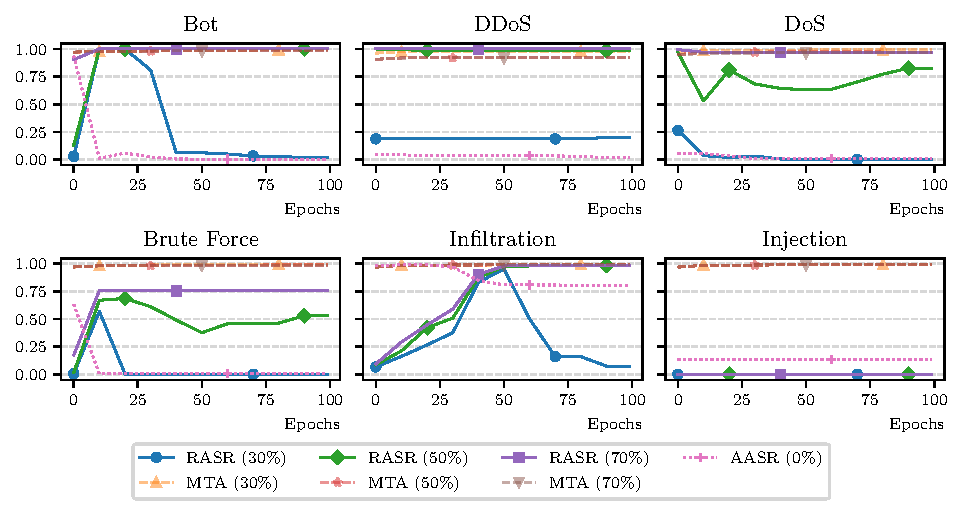
\includegraphics[width=\linewidth]{figures/cicids/backdoors}
    \caption{
      CIC-CSE-IDS2018.
      \label{fig:backdoors.cicids}
    }
  \end{subfigure}
  \begin{subfigure}{\linewidth}
    \centering
    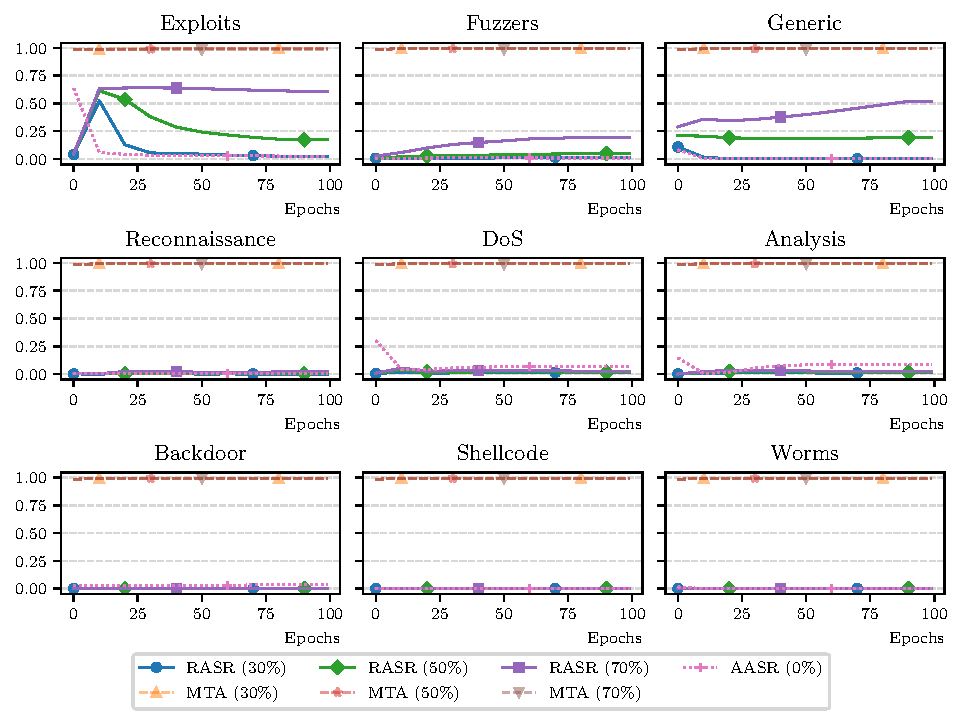
\includegraphics[width=\linewidth]{figures/nb15/backdoors}
    \caption{
      UNSW-NB15.
      \label{fig:backdoors.nb15}
    }
  \end{subfigure}
  \caption[
    \Gls{rasr} of targeted label-flipping attacks over time.
  ]{
    \Gls{rasr} of targeted label-flipping attacks over time, with $\beta=512$, $\mathcal{E}=10$, and $\alpha=1.0$.
    The $x$-axis represents the number of local epochs.
    The \gls{aasr} of the benign scenario is provided as a reference for each targeted class.
    \label{fig:backdoors}
  }
\end{figure}

\Cref{fig:backdoors} presents the impact of label-flipping attacks on the accuracy of the global model for different attack targets.
The figures show the \gls{rasr} of targeted attacks towards the different classes available in each dataset.
To measure the impact of the attack on the model's overall performance, we also measure the \gls{mta} under the differnet attacks.
The \gls{aasr} of the benign scenario is provided as a reference (\cf \Cref{fig:assess.baseline}).

The first striking observation is that the results differ greatly between the two datasets.
While on \texttt{cicids}, some attacks can reach an \gls{asr} close to 1.0 given enough attackers, most results on \texttt{nb15} remain below 0.25.
Some classes seem completely immune to the attack, such as ``Backdoor'', ``Shellcode'', and ``Worms''.
Even the most successful attacks on \texttt{nb15} barely exceed 0.5.
On \texttt{cicids}, on the other hand, the results are more convincing.
While 30\% of attackers are not enough to permanently impact the global model's accuracy, multiple classes can reach an \gls{rasr} close to 1.0 at least momentarily.
With $\tau=0.5$, the \gls{rasr} of ``Bot'', ``DDoS'', and ``Infiltation'' classes permanently reach 1.0 after a few rounds.
Most importantly, the \gls{mta} of the global model remains close to its nominal performance, even when the \gls{rasr} of the targeted classes reaches 1.0, except for the ``DDoS'' class.
Indeed, the ``DDoS'' class is the most represented in the dataset, with 5.29\% of the samples. 
Therefore, the misclassification of roughly 70\% of the samples of this class leads to a more significant impact on the global model's accuracy.

The result disparity between classes, and more importantly between datasets, is difficult to interpret, although multiple hypotheses can be formulated.
First, some classes are significantly less represented in the datasets such as ``Injection'' in \texttt{cicids} or ``Analysis'', ``Backdoor'', ``Shellcode'', and ``Worms'' in \texttt{nb15} (see \Cref{tbl:assess.datasets}).
All these targets yielded a \gls{rasr} close to 0.0.
Second, as we consider binary classification tasks, any overlap between classes' characteristics can be used by the model to infer the correct associations using samples from unaffected classes.
For instance, the ``Brute Force'' and ``DoS'' classes in \texttt{cicids} both imply a high number of connections from a single host, and both obtain subpar results when compared to the most efficient attacks.

\begin{answerbox}{Answering~\ref{rq:assess.backdoors} \normalfont\itshape\rqbackdoor}
  This type of attack has less impact on the global model's \gls{mta}, meaning that they are more likely to remain undetected.
  Although not all classes are equally impacted, \emph{\gls{ids} backdoors are possible using label-flipping attacks, given a sufficient number of attackers and a well-represented target.}
  Colluding attackers can realistically create a backdoor that may later be leveraged to evade detection, raising the question of the minimum \gls{dpr} and \gls{mpr} necessary for such attacks to be effective.
  Yet, the results are dataset-dependent, and some classes remain completely immune to the attack in our experiments.
\end{answerbox}


% ------------------------------------------------------------------------------
% RQ5: TIPPING POINT
% ------------------------------------------------------------------------------

\subsection{Threshold for Effective Attacks\label{sec:results.impact}}

\Cref{sec:assess.results.backdoors} suggests that the number of attackers is a critical factor in the effectiveness of targeted attacks.
This experiment aims to understand the critical threshold where label-flipping attacks begin to impact the global model's accuracy by studying both the \gls{dpr} ($\alpha$) and the \gls{mpr} ($\tau$).
\Cref{tbl:assess.threshold} summarizes the parameters used for this experiment.
Our previous experiments highlighted the impact of the number of attackers on the global model's accuracy.


\begin{table}
  \caption{
    Experiment parameters for \ref{rq:assess.threshold}
    \label{tbl:assess.threshold}
  }
  \small
  \begin{tabular}{>{\ttfamily\itshape}p{.2\columnwidth} >{\ttfamily}p{.7\columnwidth}}
    \toprule
    \multicolumn{2}{>{\bfseries}p{.9\columnwidth}}{\rqthreshold} \\
    \midrule
    distribution & 10-0, 9-1, 7-3, 5-5, 3-7 \\
    scenario & continuous-\{10,30,60,70,80,90,95,99,100\} \\
    target & untargeted, dos, ddos, bot, infiltration \\
    dataset & cicids, nb15 \\
    \bottomrule
  \end{tabular}
\end{table}


\begin{figure*}
  \centering
  \begin{subfigure}{\linewidth}
    \centering
    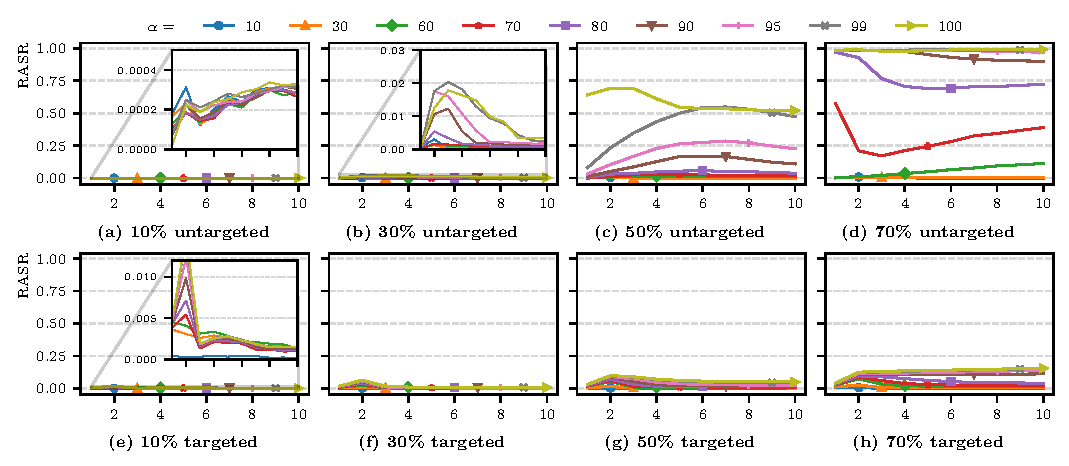
\includegraphics[width=\linewidth]{figures/cicids/attacks}
    \caption{
      CIC-CSE-IDS2018
      \label{fig:assess.threshold.cicids}
    }
  \end{subfigure}
  \begin{subfigure}{\linewidth}
    \centering
    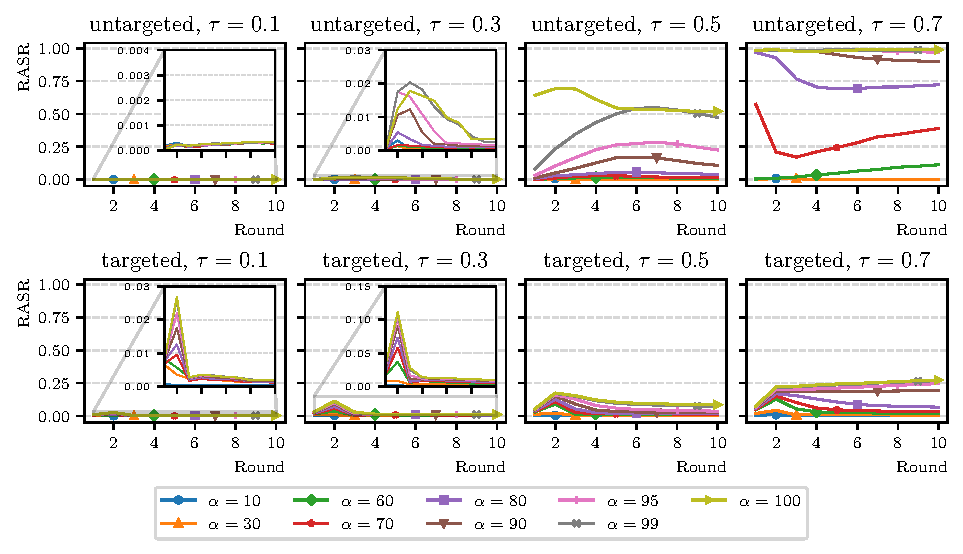
\includegraphics[width=\linewidth]{figures/nb15/attacks}
    \caption{
      UNSW-NB15
      \label{fig:assess.threshold.nb15}
    }
  \end{subfigure}
  \caption[
    Evolution of the \gls{rasr} of poisoning attacks over time, depending on the local poisoning rate ($\alpha$), the proportion of attackers ($\tau$), and the type of attack.
  ]{
    Evolution of the \gls{rasr} of poisoning attacks over time, depending on the local poisoning rate ($\alpha$), the proportion of attackers ($\tau$), and the type of attack.
    The $x$-axis represents the number of rounds.
    The value for targeted attacks is the mean of the targets, from which we exclude the under-represented and ineffective ones (see \Cref{fig:backdoors}): ``Infiltration'' and ``Injection'' in \texttt{cicids}, and ``Analysis'', ``Backdoor'', ``Shellcode'', and ``Worms'' in \texttt{nb15}.
    The \gls{fl} round is used as the time unit.
    \label{fig:assess.threshold}
  }
\end{figure*}

\Cref{fig:assess.threshold} presents the \gls{rasr} of considered label-flipping attacks over time, both for untargeted and targeted attacks.
The entire figure emphasizes on the importance of the number of attackers in the effectiveness of the attack, as most attacks are unimpactful with while $\tau \leq 0.3$.
In particular, with one single attacker ($\tau=0.1$), the \gls{rasr} remains well below 0.1, even with a high poisoning rate ($\alpha=1.0$).
$\tau=0.5$ represents a tipping point in our tests, with \gls{rasr} values orders of magnitude higher than with $\tau=0.3$.

More importantly, we can infer from $\Gamma=\tau\times\alpha$ the overall quantity of poisoned data due to our \gls{iid} partitioning.
For untargeted attacks in \texttt{cicids}, the \gls{rasr} exceeds 0.5 for $\Gamma>0.5$, and approach 1.0 for $\Gamma>0.67$.
For targeted attacks, the \gls{rasr} exceeds 0.5 for $\Gamma>0.49$ and approaches 1.0 for  $\Gamma>0.56$.
Untargeted attacks on \texttt{nb15} are slightly more effective, with the \gls{rasr} exceeding 0.5 for $\Gamma>0.49$ and approaching 1.0 for $\Gamma>0.63$.
However, as highlighted in \Cref{sec:assess.results.backdoors}, targeted attacks on \texttt{nb15} are close to ineffective, with the \gls{rasr} never exceeding 0.25, even with $\Gamma=0.7$, our highest overall poisoning rate.
Thus, \gls{rasr} and the tuple $(\alpha, \tau)$ exhibit fairly similar variations, albeit not linear: the higher the \gls{dpr} and \gls{mpr}, the higher the \gls{rasr}.
However, poisoning the entire local dataset seems more powerful than instantiating more attackers: $\alpha=100$ and $\tau=50$ yield higher \gls{rasr} than $\alpha=80$ and $\tau=70$, although the latter represents more affected data overall.

\begin{answerbox}{Answering~\ref{rq:assess.threshold} \normalfont\itshape\rqthreshold}
  The effectiveness of label-flipping attacks is directly related the overall quantity of poisoned data.
  However, this relationship is not linear, and there is a critical threshold when $\alpha$ is below 1.0.
  \Gls{fl} suffers from same caveat as numerous other distributed systems, where the majority of participants must be honest to ensure the system's security.
  \emph{However, even in its default configuration and without any defense mechanisms, multiple attackers are necessary to impact the global model's accuracy.}
\end{answerbox}


% ------------------------------------------------------------------------------
% RQ6: SIMILARITY
% ------------------------------------------------------------------------------

\subsection{Similarity as a Defense Mechanism\label{sec:results.similarity}}

\begin{table}
  \caption{
    Experiment parameters for \ref{rq:assess.similarity}
    \label{tbl:assess.similarity}
  }
  \small
  \begin{tabular}{>{\ttfamily\itshape}p{.2\columnwidth} >{\ttfamily}p{.7\columnwidth}}
    \toprule
    \multicolumn{2}{>{\bfseries}p{.9\columnwidth}}{\rqsim} \\
    \midrule
    distribution & 10-0, 9-1, 5-5 \\
    scenario & continuous-100 \\
    target & untargeted \\
    partitioner & iid\_drop\_1, kmeans\_drop\_1, iid\_drop\_2, kmeans\_drop\_2, iid\_keep\_1, iid\_full, kmeans\_full, kmeans\_keep\_1 \\
    dataset & cicids, nb15 \\
    \bottomrule
  \end{tabular}
\end{table}

A significant amount of literature has been dedicated to the development of defense mechanisms against poisoning attacks.
One of the most represented strategies is the use of similarity metrics to detect poisoned contributions~\cite{fung_LimitationsFederatedLearning_2020,awan_CONTRADefendingPoisoning_2021,cao_FLTrustByzantinerobustFederated_2022,nguyen_FLAMETamingBackdoors_2022}.
This relies on assumption that the attackers' model updates are statistically different from those of benign participants, and that a profile of either of those can be established.
For instance, \textcite{tolpegin_DataPoisoningAttacks_2020} propose to use \gls{pca} to measure the distance between model updates in the projected space.
To assess the effectiveness of this strategy for \glspl{cids}, we explore the impact of different partitioning schemes (\cf \Cref{sec:assess.method.partition}) on the \gls{pca} analysis.
\Cref{tbl:assess.similarity} summarizes the parameters used for this experiment.

\begin{figure}
  \centering
  \begin{subfigure}[t]{0.48\linewidth}
    \centering
    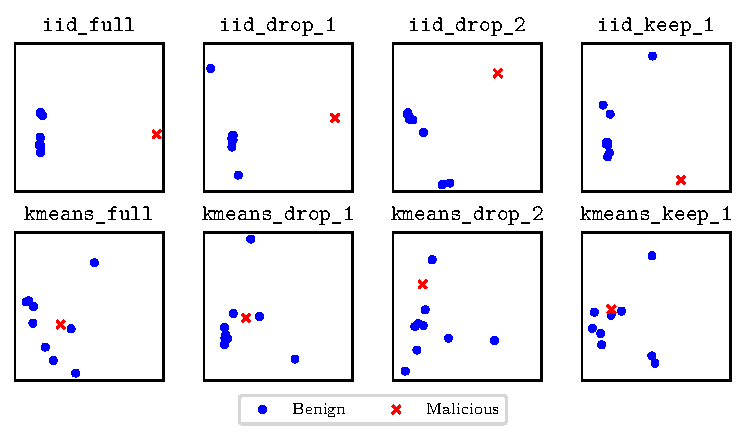
\includegraphics[width=\linewidth]{figures/cicids/similarity-untargeted-single}
    \caption{
      Single attacker on CIC-CSE-IDS2018
      \label{fig:assess.similarity.single-cicids}
    }
  \end{subfigure}
  \hfill
  \begin{subfigure}[t]{0.48\linewidth}
    \centering
    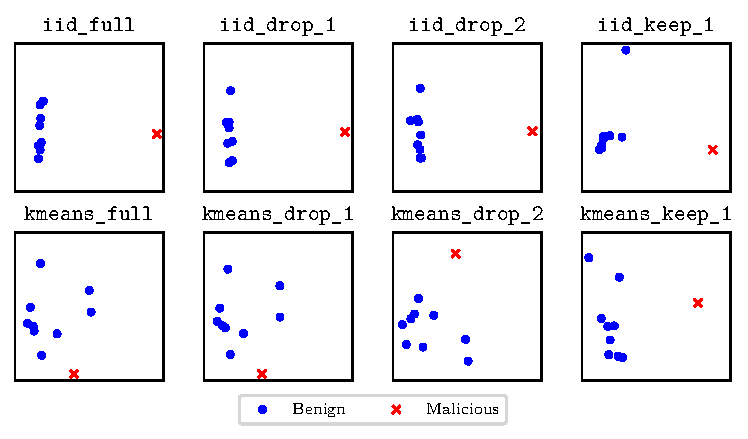
\includegraphics[width=\linewidth]{figures/nb15/similarity-untargeted-single}
    \caption{
      Single attacker on UNSW-NB15
      \label{fig:assess.similarity.single-nb15}
    }
    \vspace{\baselineskip}
  \end{subfigure}

  \begin{subfigure}[t]{0.48\linewidth}
    \centering
    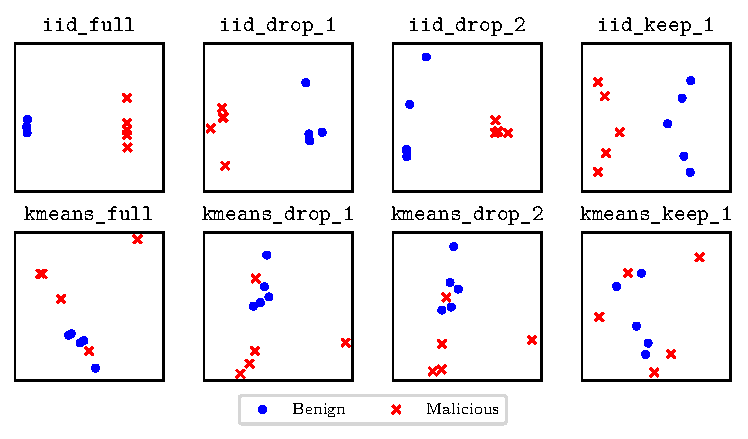
\includegraphics[width=\linewidth]{figures/cicids/similarity-untargeted-colluding}
    \caption{
      Colluding attackers on CIC-CSE-IDS2018
      \label{fig:assess.similarity.colluding-cicids}
    }
  \end{subfigure}
  \hfill
  \begin{subfigure}[t]{0.48\linewidth}
    \centering
    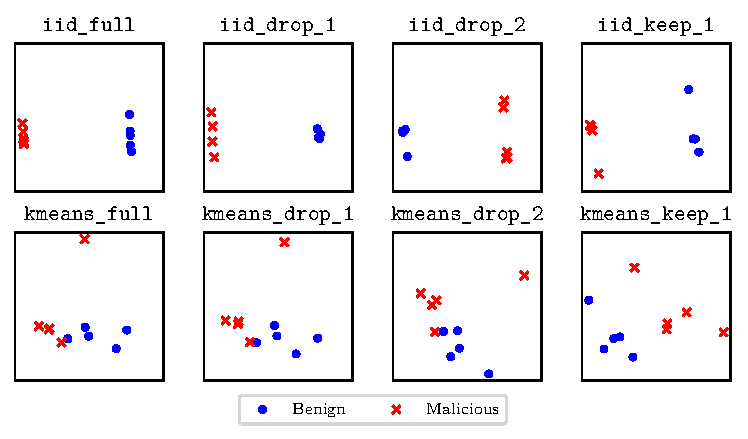
\includegraphics[width=\linewidth]{figures/nb15/similarity-untargeted-colluding}
    \caption{
      Colluding attackers on UNSW-NB15
      \label{fig:assess.similarity.colluding-nb15}
    }
  \end{subfigure}
  \caption[
    2D projection of gradients using \gls{pca} for different partitioning schemes.
  ]{
    2D projection of gradients using \gls{pca} for different partitioning schemes.
    The top row represents the results for a single attacker (\ie, $\tau=0.1$), while the bottom row illustrates the results for colluding attackers (\ie, $\tau=0.5$).
    Results for the 10\textsuperscript{th} round with \texttt{seed=1128} and $\alpha=1.0$. 
    \label{fig:assess.similarity}
  }
\end{figure}


\Cref{fig:assess.similarity} presents 2D projections of the participants' gradients using \gls{pca} for different partitioning schemes.
Each point represents a client's contribution to the global model's update at the 10\textsuperscript{th} round.
Since \texttt{FedAvg} aggregates models by default, we compute the gradients $g_i^r$ as the difference between the participant's model at round $r$ and the last global model, \ie,
\begin{equation}
  g_i^r = \bar{w}^{r-1} - w_i^r.
\end{equation}
This allows us to compare the participants' \emph{direction}, rather than their \emph{position} in the model's parameter space.

The results on the \verb|iid_full| setting are consistent with the literature: the benign participants' contributions are tightly clustered, and the attacker's contributions are easily identifiable as outliers~\cite{tolpegin_DataPoisoningAttacks_2020}.
However, the more heterogeneous partitioning schemes make it less clear, especially with a single attacker.
For instance, the \verb|kmeans_keep_1| partitioning scheme on \texttt{cicids} (\Cref{fig:assess.similarity.single-cicids}) displays two outliers that are approximately as far from the benign participants, one of which is the attacker.
In the \verb|kmeans_*| schemes, the attacker is sometime s indistinguishable from the benign participants.
Colluding attackers are more easily identifiable, as they are usually grouped together in the less heterogeneous settings.
This quality disappears with the \verb|kmeans_*| schemes, especially with \texttt{cicids} (\Cref{fig:assess.similarity.colluding-cicids}).
The two datasets exhibit slightly different behaviors, with attackers being more easily identifiable on \texttt{nb15} than on \texttt{cicids}, depending on the partitioning scheme.

\begin{answerbox}{Answering~\ref{rq:assess.similarity} \normalfont\itshape\rqsim}
  The \gls{pca} analysis provides an easy and visual way to detect attackers, as long as the data distribution is homogeneous enough.
  However, this defense mechanism is particularly challenged in more heterogeneous settings.
  Colluding attackers are more easily identifiable as they will usually form a cluster of their own, highlighting the relevance of mitigation strategies such as \texttt{FoolsGold}~\cite{fung_LimitationsFederatedLearning_2020} and \texttt{CONTRA}~\cite{awan_CONTRADefendingPoisoning_2021} which detect colluding attackers in heterogeneous environments using their similarity.
  Overall, \emph{similarity-based defense mechanisms are effective in detecting attackers in homogeneous environments, but their effectiveness decreases with the heterogeneity of the data distribution.}
\end{answerbox}